\documentclass{article}

\usepackage{amsmath}
\usepackage{graphicx}
\usepackage{pgfplots}
\usepackage[utf8]{inputenc}

\DeclareMathOperator\erf{erf}
\DeclareMathOperator\Reynolds{Re}

\title{Homework 1}

\author{Crist\'obal Armaza, Heather Wilber, Chris Silvia}

\begin{document}

\maketitle

\section{Partners}

We found our partners. We met and figured out solutions to the problems together, including investigating MPI.  We then split up the work of writing up the solutions. Christopher wrote the solution to problem 2, Crist\'obal wrote the solution to problem 3, and Heather wrote the solution to problem 4. We co-edit each other's work and have started a Github repo where we can work collaboratively on one document. 

\section{Free Shear Flows}

In this section, we investigate two types of 2D free shear flows:
	the splitter-plate and the wake.
In the splitter-plate, two flows of different velocity are separated by
	a splitter, until they meet and mix.
In the wake, interactions with an obstacle cause a region of reduced
	velocity behind an object, and this region of reduced
	velocity spreads and diffuses as the fluid continues onwards.

\subsection{Deriving the Governing Equations}

To begin our analysis of 2D shear flows, we need to determine exactly 
	which partial differential equations and boundary conditions
	we need to use.

\subsubsection{Simplifying Navier-Stokes for 2D free shear flow}

The 2D navier-stokes equations for a newtonian fluid are:

\begin{align}
\partial_t \rho + \partial_i \left( \rho u_i \right) & = 0 \\
\partial_t \left( \rho u_i \right) + \partial_j \left( \rho u_i u_j \right)
	& = - \partial_i p + \partial_j \tau_{ij} + \rho g_i\\
\tau_{ij} & = \mu \left( \partial_i u_j + \partial_j u_i \right)
\end{align}

Suppose our experiment is taking place in a thin region between two
	flat frictionless plates, and that the plates are placed horizontally.
If our velocities are not too high, and the material properties are not
	expected to change drastically, we can thus assume constant
	density and constant viscosity.
Since our experiment is between two plates, all velocities are two-dimensional
	velocities.
Since our plates are placed horizontally, with a very small height,
	the body forces are not going to cause a significant difference
	in pressure, and can thus be neglected.
Similarly, since our plates are placed horizontally, and the region
	of interest is very thin, and we assume that a constant pressure
	from the atmosphere is applied on both sides of the plates,
	then we can assume that the pressure within the region of 
	interest is constant.

If we neglect body forces, we can drop the $\rho g_i$ term.
Similarly if we neglect pressure forces, we can drop the $\partial_i p$ term.

If we assume constant density, we can simplify the mass-conservation
	equations drastically, and we can also simplify the momentum 
	equation by dividing by density. 
When density is constant, the mass conservation equation simply becomes
	$\partial_i u_i = 0$.

This will also have an impact on the momentum equation. 
The convection term is given by the following expression:
	$\partial_j \left( u_i u_j \right) =
	\left( \partial_j u_i \right) u_j 
	+ u_i \left( \partial_j u_j \right)$.
Since we found that constant density implied that $\partial_j u_j = 0$,
	we can drop the second term and just write $u_j \partial_j u_i$.

If we assume constant viscosity, we can move the viscosity out of the 
	derivative of the deviatoric stress $\tau$.
Now, $\partial_j \tau_{ij} = \mu \left( \partial_i 
	\left( \partial_j u_j \right) + \partial_j \partial_j u_i \right)$.
Since we found that constant density implied $\partial_j u_j = 0$,
	we can thus conclude that $\partial_j \tau_{ij} 
	= \mu \partial_j \partial_j u_i$.

The navier-stokes equations now become ($\nu = \frac{\mu}{\rho}$):

\begin{align}
\partial_i u_i & = 0 \\
\partial_t u_i + u_j \partial_j u_i & = \nu \nabla^2 u_i
\end{align}

\subsubsection{Boundary conditions}

The boundary conditions for our flows are different in the temporally-
	evolving limit than they are in the rest frame.

In the rest frame, for the splitter-plate, the boundary conditions are that
	there is a no-slip condition at the splitter-plate.
Before the splitter plate, on either side, there are inlet boundary
	conditions with a fixed velocity.
Below and above the splitter plate, the boundary conditions are that
	infinitely below the splitter plate the velocity
	assumes the value of the velocity in the lower inlet,
	and infinitely above the splitter plate the velocity
	assumes the value of the velocity in the upper inlet.
There is no boundary condition far to the right of the region of interest,
	i.e., it is an "exit" boundary condition.

In the rest frame, for the wake, we assume that the object producing the
	wake is not in the region of interest.
We then have to the have the inlet boundary condition, to the left,
	be the velocity profile downstream of an object.
The upper and lower boundary conditions, at effective infinity, 
	are that the velocity is the stream velocity.
The right boundary conditions is an "exit" boundary condition.

For the moving frames, where the spatial to temporal approximation is made,
	the boundary conditions are similar but different.
For both situations, uniformity in $x$ is assumed, so that we only
	have to worry about variations in $y$.

For the temporally-evolving splitter-plate case, our boundary condition
	is, if the velocity deficit between the two streams is $2 U$,
	the velocity at $y=-\infty$ is $-U$, and the velocity at
	$y = \infty$ is $U$.

For the temporally-evolving wake case, our boundary conditions is that
	the velocity deficit goes to $0$ at both $y = -\infty$ and 
	at $y=\infty$.

\subsection{Mixing Layer Solution}

By deciding to move in a reference frame which moves with the average fluid
	velocity, the mixing layer problem is simplified.
Instead of the two fluids moving with large velocities, with their velocities
	being slightly different, in the moving reference frame the two fluids 
	move in opposite directions.
The faster fluid moves with velocity $U\hat{x}$ in the moving
	frame, and the slower fluid moves with velocity $-U\hat{x}$.
The price we pay for this misdirection is that the relative fluid velocities
	must be small.
An intuitive reason for this being the case is that for the mixing
	to be time-evolving, the two fluids must be carried away from the
	splitter far faster then the timescale on which they mix.

Since we're in a moving reference frame, the spatially-and-temporally
	propagating problem from before now reduces just to a temporally
	evolving system.
Since the fluid is moving much faster than the relative velocities,
	we can assume that any non-uniformities along the direction
	of flow are on much larger scales than in the direction
	between the two fluids.
We can therefore assume that the fluid is identical in the $x$ 
	direction.

We assume that at time $t=0$, when the fluids just pass the splitter-plate,
	the fluid above $y=0$ is all moving with velocity $U \hat{x}$,
	and the fluid below $y=0$ is all moving with velocit $-U \hat{x}$.
Since the velocities are small, as assumed before, \emph{we can neglect the
	convective term}, which is quadratic in velocity.
Since the velocity we care about is the velocity in the $\hat{x}$ direction,
	and we only see it varying along $y$, we can write this as 
	$u(y)$ and consider only the diffusion of $u$ along $y$ over time:

\begin{align}
\frac{\partial u}{\partial t} & = \nu \frac{\partial^2 u}{\partial y^2}
\end{align}

As for initial conditions, we assume that because of whatever physics
	occurs at the splitter plate, the initial conditions are
	not an exact step function, but follow the following 
	profile:

\begin{align}
u(y,t=0) & = U \erf \left( \frac{ \sqrt{\pi} y}{\delta } \right)
\end{align}

We will attack this problem with the Fourier transform.
We will use the convention where $\mathcal{F}(f(x))(\xi) =
	 \int f(x) e^{-2 \pi i \xi y} dx$.
With this convention, $\mathcal{F} \left(\partial_y u(y)\right) 
	= 2\pi i \xi \hat{u}(\xi)$
Thus, $\mathcal{F} \left(\partial_y^2 u(y)\right) 
	= - 4 \pi^2 \xi^2 \hat{u}(\xi)$.

We can now write the PDE, transformed to $\xi$-space, and its solution
	for different values of $t$:

\begin{align}
\partial_t \hat{u}(\xi, t) & = - 4 \pi^2 \nu \xi^2 \hat{u}(\xi, t) \\
\hat{u}(\xi, t) & = \exp \left( - 4 \pi^2 \xi^2 \nu t \right) \hat{u}(\xi, 0)
\end{align}

Since we know $u(x,0)$, we can find $\hat{u}(\xi, 0)$.
Since we know the fourier transform of $f(a x)$ if we know the
	fourier transform of $f(x)$, we can find the fourier
	transform of $f(a x)$. 

\begin{align}
\mathcal{F}(\erf(x))(\xi) & = 
	\frac{-i}{\pi \xi} \exp \left(\pi^2 \xi^2 \right)\\
\mathcal{F}(f(a x))(\xi) & = 
	\frac{1}{a} \mathcal{F}(f(x))\left(\frac{\xi}{a}\right)\\
\mathcal{F}(\erf(a x))(\xi) & =
	\frac{-i}{\pi \xi} \exp \left(\pi^2 
		\left( \frac{\xi}{a} \right)^2 \right)
\end{align}

Since $u(x,0) = U \erf \left( \frac{\sqrt{\pi}}{\delta} y \right) $,
	the fourier transform of $u(x, 0)$ is:

\begin{align}
\hat{u}(\xi, 0) & = u
	\frac{- i }{\pi \xi}\exp \left(-\pi^2 
		\left( \frac{\xi}{\frac{\sqrt{\pi}}{\delta}} \right)^2 \right)\\
\hat{u}(\xi, t) & = 
	\exp \left( - 4 \pi^2 \xi^2 \nu t \right) \hat{u}(\xi, 0) \nonumber \\
& = U
	\frac{- i }{\pi \xi}\exp \left(-\pi^2 \xi^2 
		\left( \frac{\delta^2}{\pi}
		+ 4 \nu t \right) \right) \nonumber\\
\hat{u}(\xi, t) &  = U \frac{- i}{\pi \xi} 
	\exp\left(- \pi^2 \left( \frac{\xi}{\frac{\sqrt{\pi}}{
	\sqrt{\delta^2 + 4 \pi \nu t}}} \right)^2 \right)
\end{align}

We can do an inverse fourier transform, using the formula for the fourier
	transform of $\erf$, to get:

\begin{align}
u(y,t) & = U \erf \left( y \frac{\sqrt{\pi}}
	{\sqrt{\delta^2 + 4 \pi \nu t}} \right) \nonumber \\
u(y,t) & = U \erf \left( \frac{ \sqrt{\pi} y}{\delta} 
	\sqrt{ \frac{\delta^2}{\delta^2 + 4 \pi \nu t}} \right) 
\end{align}

\subsubsection{Vorticity Thickness}

We can define the vorticity thickness $\delta_w$ as:

\begin{align}
\delta_w & = \frac{\Delta U}{\left( \partial u / \partial y \right)_\text{max}}
\end{align}

The derivative of $\erf$ is $\partial_x \erf(x) 
	= \frac{2}{\sqrt{\pi}} e^{-x^2}$.
Thus:

\begin{align}
\partial u / \partial y & = \frac{2 U}{\sqrt{\pi}} 
	\exp \left( - \left( \frac{ \sqrt{\pi} y}{\delta} 
	\sqrt{ \frac{\delta^2}{\delta^2 + 4 \pi \nu t}} \right)^2 \right) 
	\frac{ \sqrt{\pi}}{\delta} 
	\sqrt{ \frac{\delta^2}{\delta^2 + 4 \pi \nu t}} \nonumber \\
\left( \partial u / \partial y \right)_\text{max} & =
	2 U \frac{1}{\delta} \frac{1}{\sqrt{1 + \frac{4 \pi \nu}{\delta^2} t}}\\
\delta_w & = \delta \sqrt{ 1 + \left( \frac{4 \pi \nu}{\delta^2} \right) t } 
\end{align}

We can see that in the limit of zero viscosity, $\delta_w = \delta$.

\subsection{Wake}

To solve the wake problem, we will follow the same general procedure
	as before.

\begin{align}
u(y,0) & = -U\exp\left(-\frac{\pi y^2}{\delta^2} \right)\\
\hat{u}(\xi, 0) & = - U \sqrt{ \frac{\pi}{\frac{\pi}{\delta^2}}}
	\exp \left( - \frac{ (\pi \xi)^2}{ \frac{\pi}{\delta^2}} \right)
	\nonumber \\
\hat{u}(\xi, 0)& = - U \delta \exp \left( - 
	\pi \left( \delta \xi \right)^2 \right) \\	
\hat{u}(\xi, t) & = - U \delta 
	\exp \left( - \pi \left( \delta \xi \right)^2 \right)
	\exp \left( - 4 \pi^2 \xi^2 \nu t \right) \nonumber\\
\hat{u}(\xi, t) & = - U \delta
	\sqrt{ \frac{\frac{1}{ \frac{\delta^2}{\pi} + 4 \nu t}}{\pi}}
	\sqrt{ \frac{\pi}{ \frac{1}{ \frac{\delta^2}{\pi} + 4 \nu t}}}
	\exp \left( - \frac{ ( \pi \xi )^2}
	{ \frac{1}{ \frac{\delta^2}{\pi} + 4 \nu t}} \right) \nonumber\\
u(y, t) & = - U \sqrt{ \frac{\delta^2}{ \delta^2 + 4 \pi \nu t}}
	\exp \left( \frac{-\pi y^2}{ \delta^2 + 4 \pi \nu t} \right)
\end{align}

The wake half-width $b$ is defined as the width between the centerline
	and the point where the velocity profile drops to half its
	maximum deficit value.
If the velocity profile is proportional to $\exp(-a x^2)$, this point occurs
	where $\exp(-a b^2) = 1/2$.  
This occurs at $b = \sqrt{\frac{\log 2}{a}}$.
In the velocity profile above, $a(t) = \frac{\pi}{\delta^2 + 4 \pi \nu t}$.
Thus:

\begin{align}
b(t) & = \sqrt{ \frac{ \log 2}{\pi} \left( \delta^2 + 4 \pi \nu t \right) }
\end{align}

In the case of no viscosity, $b = \delta \sqrt{\frac{\log 2}{\pi}}$

\subsubsection{Interpretation as Position, Dimensionless Quantities}

If we go back to the static reference frame, we can equate time and downstream
	$x$ position via the identity $x = V t$, where $V$ is the free
	stream velocity.
We can thus transform $b(t)$ into $b(x)$ in the rest frame:

\begin{align}
b(x) & = \delta \sqrt{\frac{\log 2}{\pi}} \sqrt{1 + \frac{4 \pi \nu}{\delta^2 V} x}
\end{align}

We can make a substitution here: the Reynolds number $\Reynolds$ is given by
	$\Reynolds = \frac{\delta V}{\nu}$, where $V$ is the velocity scale
	and $\delta$ is the length scale.
We can find the reyonlds number in the formula:

\begin{align}
b(x) & = \delta \sqrt{\frac{\log 2}{\pi}} 
	\sqrt{1 + \frac{4 \pi}{\Reynolds} \frac{x}{\delta}}
\end{align}

%question 3
\section{Parallelism}

\subsection{Parts (a) and (b)}
We installed the corresponding libraries on our machines.
 
\subsection{Part (c)} 
After running \textit{hello\_world.f90}, we succeeded in getting the message
\begin{verbatim}
Hello, my processor rank is           0
\end{verbatim}
Then, we increased the number of processors and got a list showing the rank of all the processors. For example,
for \textit{-np 10}, the list was
\begin{verbatim}
Hello, my processor rank is           0
Hello, my processor rank is           1
Hello, my processor rank is           5
Hello, my processor rank is           6
Hello, my processor rank is           9
Hello, my processor rank is           7
Hello, my processor rank is           3
Hello, my processor rank is           4
Hello, my processor rank is           8
Hello, my processor rank is           2
\end{verbatim}
After trying larger numbers, we proved that we are able to execute more processors than any of 
our machines physically has.
 
\subsection{Part (d)}
In order to explore the execution time and performance, we include the simple operation
\begin{equation}
a = \exp(5+0.001 b),
\end{equation}
where $b$ is a random number obtained at each iteration. The number of iterations is $N/$\textit{np},
with $N=10^8$. As we increase the number of processors (\textit{np}), 
the execution time in each node decreases. For example, for $np = 1, \,2,\,3$, we obtain, respectively,
\begin{verbatim}
Hello, my processor rank is 0 of 1 Processors taking 2.30102539 seconds.
 
Hello, my processor rank is 0 of 2 Processors taking 1.89941406 seconds.
Hello, my processor rank is 1 of 2 Processors taking 1.91113281 seconds.
 
Hello, my processor rank is 2 of 3 Processors taking 0.790527344 seconds.
Hello, my processor rank is 1 of 3 Processors taking 0.792480469 seconds.
Hello, my processor rank is 0 of 3 Processors taking 0.793457031 seconds.
\end{verbatim}
One thing we immediately notice is that, for a given value of \textit{np}, the execution time
varies in each node. We will come back to this later. 

The figure below shows the execution time as a function of the number of processors. On our laptop, we are able to declare up
to 199 processors before getting an error message. As expected, the execution time decreases as we declare more processors. 
The points on the plot are relatively well described by the curve $f(\text{\textit{np}}) \propto 1/\text{\textit{np}}$ 
(blue curve on the plot). This is consistent with the theoretical expectation that the time to perform a task would decrease
by \textit{np} after dividing the task among \textit{np} processors. For large ($> 100$) \textit{np}, we note that the time
ceases to decrease, and stays at a roughly constant (non-vanishing) value. Since assigning tasks to each processor takes 
some finite time, we might interpret the constant value as this assignment time such that, for large \textit{np}, this 
time dominates over the execution time in the node. We learn from this that parallelizing a program is convenient, 
as long as the task of parallelizing itself does not take longer than running the program.

When keeping all the parameters the same, we note some variations in the execution time of each processor across different
runs, and among different processors during the same run. If the nodes were processing a single task and nothing else,
we would expect the time to be equal across every node and for all of the runs. In reality, there are more
(probably many) tasks being executed in the background, which affect the individual execution time of each processor.
The bus is assigning jobs to nodes in the midst of and with respect to this variable CPU usage. This can cause the work
performed by any individual node to vary across different runs, even though the parameters are the same.

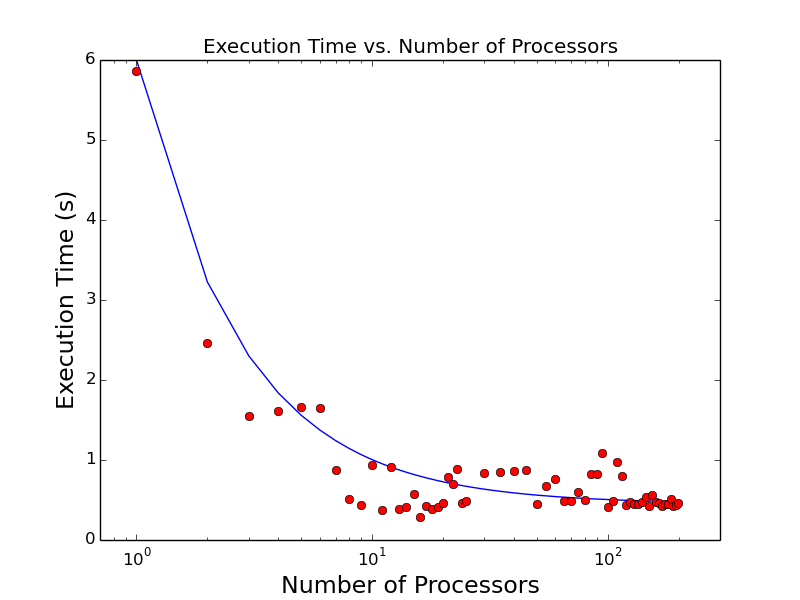
\includegraphics[width=1\textwidth]{t_vs_np.png}


%question 4
\section{ Nonuniform Mesh generation}

In this problem we generate a non-uniform 1D mesh consisting of $n$ cells between the locations $y_0$ and $y_n$. Cell $j$ is of size $\Delta y_j = y_j-y_{j-1}$, $ 1\leq j \leq n$, and cells are stretched according to $\dfrac{\Delta y_{j+1}}{\Delta y_j}  =\alpha$, where $\alpha$ is a user-provided parameter. To write a mesh-generating code, we note that 
\[ y_j  = \Delta y_j + y_{j-1} = \sum_{k=1}^{j-1} \Delta y_k + y_0.\]
Since $\Delta y_2 = \alpha \Delta y_1$, and in general $\Delta y_{j+1} = \alpha  \Delta y_{j}$, we have that $\Delta y_{j} = \alpha^{j-1} \Delta y_1$. This gives us the following formula for $y_j$:
\[ y_j  = \Delta y_j + y_{j-1} = \sum_{k=1}^{j} \alpha^{-1} \Delta y_1 + y_0, \]
which, when we sum the geometric series, can be written as 
\begin{equation}
\label{eq:yj}
 y_j = \dfrac{\alpha^{j}-1}{\alpha -1} \Delta y_1 +y_0. 
\end{equation}

\subsection{Part (a)}
Here we generate a mesh with $n=128$ using $ \alpha = 1.05$ between $y_0 = 0$ and $y_n = 1$.  We use~\eqref{eq:yj} with $(n, y_n) = (128, 1)$ to find that $ \Delta y_1 \approx 9.7181 \times 10^{-05} $.  

Below we include images of the mesh. The 1D mesh described above was generated in the $y$-direction, and we used $128$ equispaced cells between $0$ and $10$ to generate a uniform grid in the $x$-direction. This makes the mesh easier to visualize. The image was generated in MATLAB using a variant of the mesh-generating code listed below in part (c).
The left plot displays the entire mesh $y_0, y_1, \cdots y_{128}$. On the right we display only the first $50$ nodes of the mesh. 

\vspace{1cm}

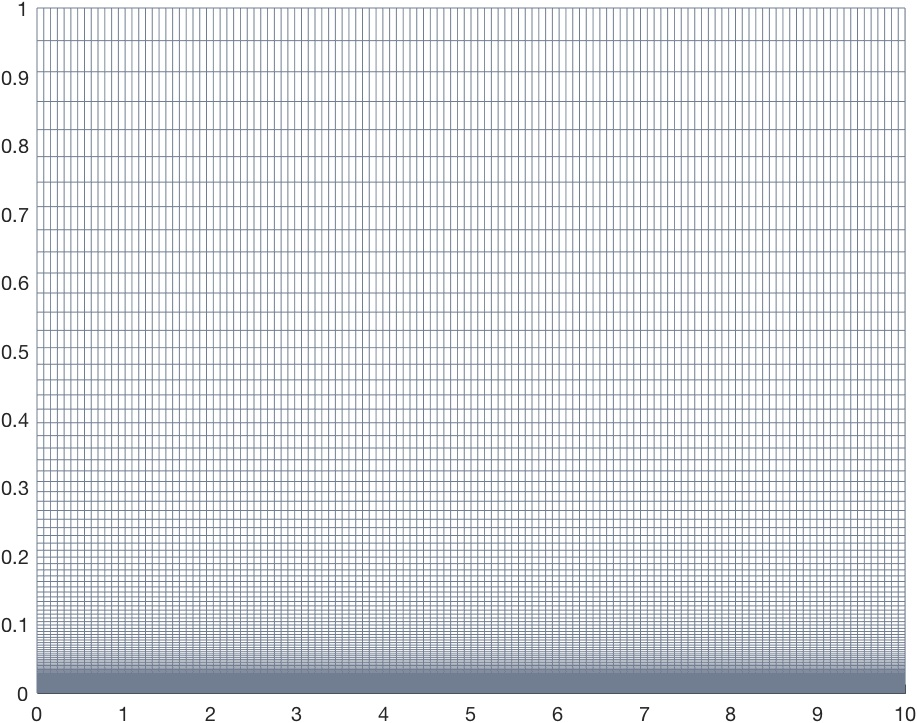
\includegraphics[width=.45\textwidth]{meshgrid.jpg} 
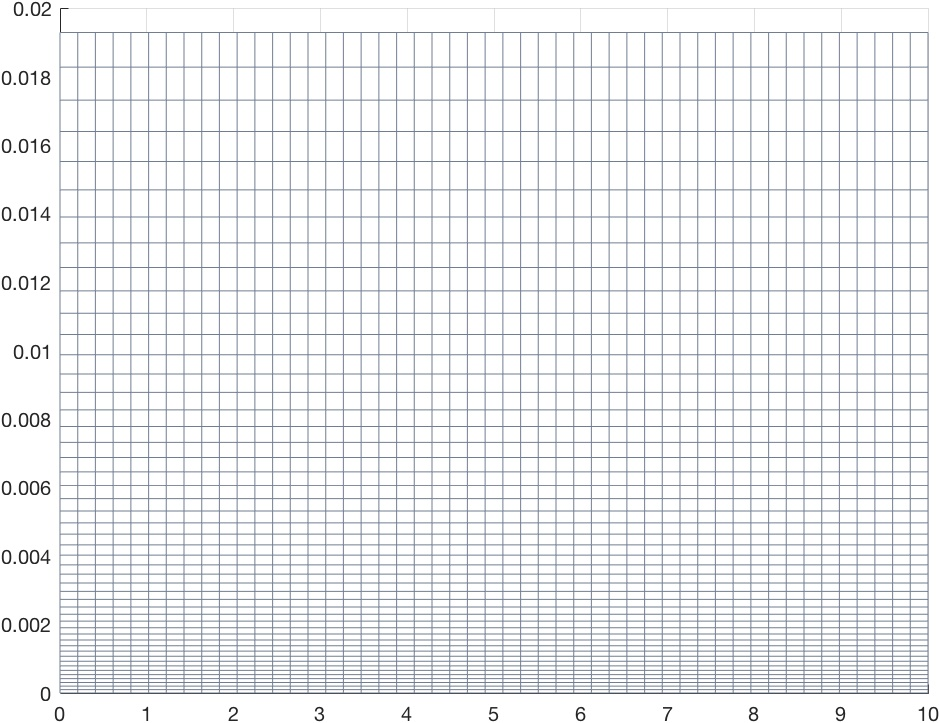
\includegraphics[width=.45\textwidth]{meshgrid_small.jpg} 

\subsection{Part (b)}
In this question, $n = 128$, $y_0 = 0$ and $y_n=1$. With $\delta_\omega = .176$, we'd like to find $\alpha$ such that $70\%$ of the grid points are concentrated between $y=0$ and $y=\delta_\omega$.  
This means that we need $y_j \leq \delta_\omega$ for $j = \lceil.7n \rceil =  90$. We choose $y_{90} = \delta_\omega$ to achieve this. We can then find the unknowns $\alpha$ and $\Delta y_1$ by plugging the values for $j = n$ and $j = 90$ into~\eqref{eq:yj} and approximately solving the resulting system of equations:
\begin{align}
& \delta_\omega = \dfrac{\alpha^{90}-1}{\alpha -1} \Delta y_1 ,\\
&  1 = \dfrac{\alpha^{128}-1}{\alpha -1} \Delta y_1 .
\end{align}
This requires an approximate solution to the equation
\begin{equation} 
\label{eq:chebeq}
(\alpha^{128} -1) \delta_\omega = \alpha^{90}-1.
\end{equation}
We find that $\alpha \approx 1.045873956297$, and subsequently, $\Delta y_1 \approx 1.4777 \times 10^{-4}$. 
We found this solution using Chebfun, a numerical computing program written in MATLAB. The Chebfun command {\tt roots} uses Chebyshev interpolants and colleague matrices to solve equations such as~\eqref{eq:chebeq} to a high degree of accuracy. Here is a printout of the Chebfun code we used: 
\begin{verbatim}
n = 128; 
d = .176;

%construct chebfuns representing eqns
y1 = chebfun(@(x) x.^n-1, [1 1.2]); 
y2 = chebfun(@(x) 1/(d)*(x.^(.7*n)-1), [1 1.2]); 

% Chebfun finds two roots, we ignore the root r(1)=1. 
r = roots(y1-y2);r = r(2); 

%find delta y1
dy1 = (r-1)./(r^n-1); 


%check results
j = ceil(.7*n); alpha = 1.05; d = 0.176;
err1 = 1- dy1*(r^128-1)/(r-1)
err2 = d- dy1*(r^(.7*128)-1)/(r-1)
\end{verbatim}
The errors, err1 and err2 are on the order of $10^{-15}$ and $10^{-10}$, respectively. 

\subsection{Part (c)}
Mesh generation code: We include the code in Fortran, as well as a variant used in MATLAB for visualization. 

(add Fortran/C code here)

\begin{verbatim}
%build the mesh
C = alpha_mesh(1.05, 0, 1, 128);

%make it 2D for better visualization. 
%this is with equispaced points in x-direction
[xx, yy]=meshgrid(linspace(0,10,129), C);
mesh(xx,yy, xx.*0+1)
view(2)
colormap(bone)
export_fig -m2 -jpg -transparent 'meshgrid'

%extract the first 50 entries
[xx2, yy2] = meshgrid(linspace(0,10, 50), C(1:50)); 
mesh(xx2, yy2, xx2.*0+1)
view(2)
colormap(bone)
export_fig -m2 -jpg -transparent 'meshgrid_small'

%..........subfunction alpha_mesh..............%

%mesh generation
% n = # cells, n+1 = # nodes
function C = alpha_mesh(alpha, y0, yn, n)
    
%find Delta y1
dy1 = (alpha-1)*(yn-y0)/(alpha^n-1);

%construct mesh
j = 1:(n-1);
C = dy1*(alpha.^j-1)./(alpha-1)+y0; 
C = [y0  C  yn];
end
\end{verbatim}




\end{document}
